\documentclass{arima-en}
% force arXiv/HAL to compile with PDFLaTeX
\pdfoutput=1 

%%%%%%%%%%%%%%%%%%%%%%%%%%%%%%%%%%%%%%%%%%%%%%%%%%%%%%%
% Modules
\usepackage{array}
\usepackage{pgfplots}
\usepackage{graphicx}
\usepackage[utf8]{inputenc}
\usepackage[T1]{fontenc}
\usepackage{fancyhdr}
\pagestyle{fancy}
\usepackage{hyperref}
\usepackage[babel]{csquotes}

%%%%%%%%%%%%%%%%%%%%%%%%%%%%%%%%%%%%%%%%%%%%%%%%%%%%%%%
% Header
\title{Prédiction du risque de crédit bancaire sensible aux coûts financiers en intégrant des descripteurs extraits des graphes}
\author[1]{Victor DJIEMBOU}
\author[1]{Armel NZEKON}
\affil[1]{Université de Yaoundé I, Cameroun} 
% corresponding author with his/her email
\corrauthor{Victor nico.djiembou@facsciences-uy1.cm, Armel armel.nzekon@facsciences-uy1.cm}

%%%%%%%%%%%%%%%%%%%%%%%%%%%%%%%%%%%%%%%%%%%%%%%%%%%%%%%
%Code for software citations
\usepackage[
  style=numeric-comp,
  datamodel=software, % extend the datamodel with entries for software
  abbreviate=false,
  natbib=true,
  sorting=ynt,
  backend=biber,
  bibencoding=utf8,
  giveninits=true,
  url=false,
  doi=false,
  defernumbers,
  maxcitenames=10,
  defernumbers=false,
  maxbibnames=100]{biblatex}
%
% Load the software biblatex style
%

\usepackage{software-biblatex}
%
% Set software specific bibliography options
%
\ExecuteBibliographyOptions{
  halid=true,
  swhid=true,
  swlabels=true,
  vcs=true,
  license=false}
%
% Make title an hyperlink to the DOI or URL to make the result leaner (suggested by N. Rougier 4/4/2020)
%

\newcommand{\doiorurl}{%
 \iffieldundef{doi}
    {\iffieldundef{url}
       {}
       {\strfield{url}}}
    {http://dx.doi.org/\strfield{doi}}%
}
\newcommand{\myhref}[1]{%
 \ifboolexpr{%
  test {\ifhyperref}
  and
  not test {\iftoggle{bbx:url}}
   and
   not test {\iftoggle{bbx:doi}}
  }
  {\href{\doiorurl}{#1}}
  {#1}%
}
\DeclareFieldFormat{title}{\myhref{\mkbibemph{#1}}}
\DeclareFieldFormat
  [article,inbook,incollection,inproceedings,patent,thesis,unpublished]
  {title}{\myhref{\mkbibquote{#1\isdot}}}
\addbibresource{ARIMA-EN.bib}



%%%%%%%%%%%%%%%%%%%%%%%%%%%%%%%%%%%%%%%%%%%%%%%%%%%%%%%
\pgfplotsset{compat=1.17}
\begin{document}
\maketitle





%%%%%%%%%%%%%%%%%%%%%%%%%%%%%%%%%%%%%%%%%%%%%%%%%%%%%%%
\abstract {
% contexte
% texte conci
%Le prêt est l'une des principales sources d'enrichissement des banques, mais est également une source de perte financière. Pour optimiser leurs profits, il est donc nécessaire pour les banques de prédire si un emprunteur remboursera ou pas son crédit. 
%% transition vers IA
%Afin d'aider les banques à aborder efficacement ce challenge, plusieurs techniques d'apprentissage automatique ont été proposées durant cette dernière décennie pour la question spécifique de prédiction du risque de crédit bancaire. 
%% transition vers graphe
%Quelques unes de ces techniques reposent sur des graphes  
%% transition vers graphes mutlicouches 
%
%% limites actuelles du graphe multicouche 
%
%% travaux réalisé pour palier les limites 
%
%% description de l'environnement d'expérimentation, jeu de données, modèles considérés, métriques d'évaluation, ...
%
%% remarques et résultats intéressants 
%
%
%L'amélioration de la capacité de ses institutions à évaluer le risque associé à une demande de prêt a été confronté à des difficultés parmi lesquelles la faible présence de données pour entraîner les modèles d'AAet la faible représentativité dans les jeux de données existant. L'analyse des comportements des emprunteurs et des liens avec leur entourage au moyen de modèles graphes a été longtemps utiliser pour augmenter les jeux de données existant avec des informations pertinentes pour combler le manque de données et relativement leur représentativité. 
%
%% objectif
%Ainsi de nombreux travaux en IA ont réussi jusqu'ici à proposer un moyen d'analyser les emprunteurs suivant deux dimensions. Différentes paires d'attributs catégorielles sont prise de façon aléatoire dans l'ensemble d'informations et sont modélisé au moyen de graphes multicouches biparti où chaque couche met les emprunteurs en relations avec la valeur d'attribut associée constituant cette couche. Ensuite des informations pertinentes comme le PageRank avec une personnalisation inter-couche, intra-couche et collective de ces graphes sont calculées via l'analyse de graphes. Néanmoins, l'aléa dans le choix d'attributs du jeu données, la limite du nombre de dimension et encore la limitation au attributs catégorielles constituent une limite car de façon hypothétique, je suis en relation avec un ensemble d'individu parce que je partage au moins une information avec cette ce groupe. 
%% méthodologie
%Alors, pour résoudre ses limites, nous adaptons d'abord l'algorithme de PageRank personnalisé multicouche pour prendre en compte unique les informations propres à un seul emprunteurs lors de la recherche d'information pertinente, ensuite nous proposons un protocole qui permet de choisir les k attributs à utiliser dans un graphe multicouche biparti à k couches, enfin les informations extraites sont intégrées dans des modèles AA notamment afin d'améliorer les métriques de classification de ses modèles. 
%% resultats
%Nous l'avons approuvé à 5 jeux de données benchmark dans le domaine du credit scoring et avons observé que nous améliorons les résultats présentent dans la littérature.

}

\keywords{risque de crédit, graphe, graphe multicouche}





%%%%%%%%%%%%%%%%%%%%%%%%%%%%%%%%%%%%%%%%%%%%%%%%%%%%%%%
\section{Introduction}
La science des réseaux s'est imposée comme une théorie fondamentale et un outil essentiel pour comprendre, modéliser et analyser les réseaux de communication. La science des réseaux s'est imposée comme une théorie fondamentale et un outil essentiel pour comprendre, décrire, modéliser et analyser les systèmes complexes d'entités en interaction qui apparaissent naturellement, par exemple, en biologie, en sociologie, en finance et en économie, parmi beaucoup d'autres [4]. Dans la vie réelle, les objets sont souvent liés par plus d'un type de relation. Par exemple, dans les réseaux sociaux en ligne, deux personnes peuvent être amies sur Facebook et se suivre sur Twitter. Ces réseaux sont généralement appelés réseaux multicouches, dont la théorie et le développement de modèles ont été au cœur de la science des réseaux au cours de la dernière décennie.

Dans le secteur bancaire, on soupçonne depuis longtemps l'existence de défaillances corrélées.
corrélées. Cependant, toutes les études qui ont porté sur la propagation du risque à travers les réseaux se sont concentrées sur la contagion.
Cependant, toutes les études portant sur la propagation du risque à travers les réseaux se sont concentrées sur la contagion entre les institutions financières [8,20] ou sur la corrélation des actifs avec l'ensemble de l'économie, proposée pour la première fois dans les accords de Bâle [5]. Plusieurs auteurs ont souligné que ces effets de corrélation affectent les mesures actuelles du risque de crédit [21,49] au niveau individuel, un fait qui a été négligé jusqu'à présent. Compte tenu de l'importance des prêts aux particuliers pour l'ensemble de l'économie et des progrès actuels de la science des réseaux, nous combinons le risque de crédit avec la science des réseaux multicouches pour présenter une méthodologie permettant de calculer explicitement l'impact de la corrélation des défaillances chez les emprunteurs connectés au niveau un à un.  Notre proposition vise donc non seulement à mieux comprendre la propagation des défaillances, mais aussi à améliorer les systèmes de notation des demandes, couramment utilisés pour prendre des décisions en matière d'octroi de prêts.

Ce document comporte trois contributions principales. Premièrement, nous présentons un
cadre pour créer un réseau bipartite multicouche à partir d'un ensemble de données tabulaires avec deux ou plusieurs variables de connexion. Ces variables ne sont pas nécessairement des variables de réseau explicites, mais peuvent être une propriété partagée ou une caractéristique. Ensuite, nous développons une nouvelle approche pour la prédiction du risque de crédit avec une mesure de centralité PageRank multicouche personnalisée qui classe les nœuds du réseau multicouche par rapport à un ensemble de nœuds sources qui peuvent être utilisés pour comprendre le risque corrélé et également pour améliorer les systèmes d'évaluation du crédit. Enfin, nous montrons que les scores d'influence des réseaux multicouches contribuent à l'amélioration des modèles d'évaluation du crédit. Bien que nos résultats soient généraux et applicables à n'importe quel ensemble de données de prêt (et à n'importe quel problème dans lequel des effets corrélés sont suspectés), nous motivons le travail dans un environnement dans lequel le risque de crédit est le plus élevé.
motivons notre travail dans un environnement où la corrélation des défaillances est évidente.
est évidente. Nous concentrons notre attention sur les réseaux multicouches dans les prêts agricoles et présentons des algorithmes généraux pour les inclure dans tout modèle prédictif où ils apparaissent. Si les réseaux multicouches ont été étudiés dans le secteur bancaire, jusqu'à présent - et à notre connaissance - leurs effets sur les prêts de détail (prêts à la consommation traditionnels et prêts de gré à gré aux petites et moyennes entreprises) n'ont pas fait l'objet du même niveau d'attention. Cela n'est pas surprenant compte tenu de sa structure : les prêts aux particuliers sont beaucoup plus nombreux, de sorte que toute interaction entre les réseaux nécessite une analyse complexe qui n'est devenue réalisable qu'au cours de la dernière décennie. Cela dit, il est également naturel de s'attendre à ce que les emprunteurs soient connectés de nombreuses manières complexes, de sorte que l'analyse utilisée pour mesurer leur comportement devrait également suivre ce niveau de complexité. 









%%%%%%%%%%%%%%%%%%%%%%%%%%%%%%%%%%%%%%%%%%%%%%%%%%%%%%%
\section{Section}
%%%%%%%%%%%%%%%%%%%%%%%%%%
\subsection{Sub-section 1}
Pellentesque dignissim ultrices fringilla. Vivamus eu luctus ante, vel bibendum magna. Curabitur elit purus, tincidunt non dui vitae, elementum bibendum neque. Curabitur ullamcorper sit amet justo at hendrerit. Fusce ut arcu imperdiet nibh mollis tempus a aliquet tellus. Quisque pharetra cursus nisi, vel lobortis ante consectetur et. Vivamus sed congue neque. Proin pellentesque risus nec dui consequat rutrum. Vestibulum nunc diam, placerat quis auctor vel, faucibus non justo. Etiam dictum purus neque. Phasellus imperdiet mauris ligula, eu laoreet nisi elementum ut. Sed sed porta massa. Aenean faucibus risus ultrices ornare porta. Quisque faucibus ante a tincidunt vestibulum. Lorem ipsum dolor sit amet, consectetur adipiscing elit.


%%%%%%%%%%%%%%%%%%%%%%%%%%
\subsection{Sub-section 2}
%%%
\subsubsection{Sub-sub-section}
Suspendisse vel dui nec felis molestie tincidunt. Vestibulum rutrum ligula lacus, ac molestie nulla fermentum ornare. Nulla non nunc euismod, porta lacus vestibulum, malesuada massa. Curabitur massa eros, rutrum sed lectus sed, volutpat semper metus. Mauris hendrerit aliquam commodo.  Vivamus fermentum tempus pellentesque. Maecenas a hendrerit urna. In elit ipsum, ultrices non dolor in, pulvinar porttitor lacus. Nunc euismod nibh quis odio condimentum, a feugiat massa rutrum. Nulla erat erat, adipiscing vitae lectus id, consectetur fermentum elit. Nunc eu est eu neque dapibus semper. Nam commodo urna dapibus, tincidunt turpis a, cursus sem. Vivamus venenatis adipiscing mollis. Cras fringilla sodales lobortis. Aliquam aliquet felis id est cursus auctor. Duis sodales tellus vulputate lectus egestas volutpat.





%%%%%%%%%%%%%%%%%%%%%%%%%%%%%%%%%%%%%%%%%%%%%%%%%%%%%%%
\section{Tables and Figures}
%%%%%%%%%%%%%%%%%%%%%%%%%%
\subsection{Tables}
Cf. Table~\ref{tab:example}.

\begin{table}[H]
  \newcolumntype{+}{>{\global\let\currentrowstyle\relax}}
  \newcolumntype{^}{>{\currentrowstyle}}
  \newcommand{\rowstyle}[1]{\gdef\currentrowstyle{#1}%
    #1\ignorespaces
  }
  \centering
  \begin{tabular}{+>{\bfseries}l^c^c^c^c}
    \hline
    \rowstyle{\bfseries}
    & S-Length & S-Width & P-Length & P-Width\\
    Setosa & 5.006 & 3.428 & 1.462 & 0.246\\
    Versicolor & 5.936 & 2.77  & 4.26  & 1.326\\
    Verginica & 6.588 & 2.974 & 5.552 & 2.026\\
    \hline
  \end{tabular}
  \caption{Morbi malesuada diam at magna condimentum.}
  \label{tab:example}
\end{table}

\subsection{Figures}

If possible, bring figures together in a block. Use images at least 300 dpi. Check that caption are legible and in english. See this example : Figure~\ref{fig:example} (from  \url{http://www.texample.net/tikz/examples/pgfplots/}). The title must be ended with a dot.


%%%%%%%%%%%%%%%%%%%%%%%%%%
\begin{figure}[H]
  \centering
  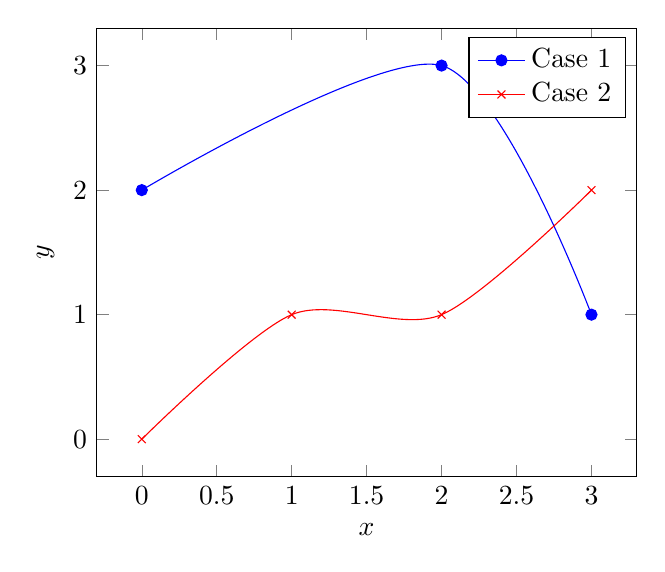
\begin{tikzpicture}
    \begin{axis}[
        xlabel=$x$,
        ylabel=$y$]
    \addplot[smooth,mark=*,blue] plot coordinates {
        (0,2)
        (2,3)
        (3,1)
    };
    \addlegendentry{Case 1}
    \addplot[smooth,color=red,mark=x]
        plot coordinates {
            (0,0)
            (1,1)
            (2,1)
            (3,2)
        };
    \addlegendentry{Case 2}
    \end{axis}
    \end{tikzpicture}
  \caption{figure de Christian Feuers\"anger; source: Pgfplots.}
  \label{fig:example}
\end{figure}

\begin{figure*}[ht] 
\resizebox{10cm}{9cm}
  {\includegraphics[width=11cm]{Lion.jpeg}}
  \centering
  \label{frog}
  \caption{Cameroon Lion (photo credit: Fist name Surname).}
  \end{figure*}
  




%%%%%%%%%%%%%%%%%%%%%%%%%%%%%%%%%%%%%%%%%%%%%%%%%%%%%%%
\section{Definitions, Algorithms and Formulas}
%%%%%%%%%%%%%%%%%%%%%%%%%%
\subsection{Definitions}
For formulas, use the package \texttt{amsthm} and the style \texttt{arima} for reliable formatting.

\begin{definition}[alpha]
Curabitur ullamcorper sit amet justo at hendrerit.
\end{definition}

Then we set the following definition.

\begin{definition}
Etiam sed nulla viverra, ultrices ligula ac, consectetur libero.
\end{definition}

For a list, use "bullets" or em dash:
\begin{itemize}
  \item Nunc id justo scelerisque ;
  \item metus id enim iaculis tristique.
\end{itemize}


%%%%%%%%%%%%%%%%%%%%%%%%%%
\subsection{Formulas}
Formulas Example:
\begin{equation}
  Y=M.^tM-\beta.\langle M \rangle_l
\end{equation}

where $\langle M \rangle_l$ is the mean vector of a $M$. $\beta$ enables the rate of close neighbours to be regulated.

Other formulas example:
\begin{equation}
  K * N_c = Cst \pm 0.001\%
\end{equation}


%%%%%%%%%%%%%%%%%%%%%%%%%%
\subsection{Algorithms}
For algorithms, use appearance of Algorithm~\ref{lst:example}. If necessary, see the package \texttt{listings}.

\begin{listing}[H]
  \begin{lstlisting}
  partition(array, left, right)
     pivotIndex := choose-pivot(array, left, right)
     pivotValue := array[pivotIndex]
     swap array[pivotIndex] and array[right]
     storeIndex := left
     for i from left to right - 1
         if array[i] < pivotValue
             swap array[i] and array[storeIndex]
             storeIndex := storeIndex + 1
     swap array[storeIndex] and array[right]  // Move pivot to its final place
     return storeIndex
  \end{lstlisting}
  \caption{Partitioning function of a sorting algorithm.}
  \label{lst:example}
\end{listing}





%%%%%%%%%%%%%%%%%%%%%%%%%%%%%%%%%%%%%%%%%%%%%%%%%%%%%%%
\section{Conclusion and references}

%%%%%%%%%%%%%%%%%%%%%%%%%%
\subsection{Discussion}
Nam id eros massa. Fusce luctus purus a augue ullamcorper, sit amet vehicula mauris tristique. Suspendisse eget pulvinar odio, nec bibendum turpis. Nullam quis lectus porttitor, ullamcorper nisi et, condimentum leo. Quisque sed orci fermentum, rutrum velit eget, ultricies augue. Nunc porttitor consectetur tincidunt. Nulla tincidunt justo enim, vitae dignissim erat mattis ut. Nulla.


%%%%%%%%%%%%%%%%%%%%%%%%%%
\subsection{Conclusion}
Maecenas egestas metus id enim iaculis tristique. Etiam sed nulla viverra, ultrices ligula ac, consectetur libero. Nullam vitae massa ac odio pharetra condimentum. Maecenas in elementum libero, non gravida quam. Praesent adipiscing consectetur consectetur. Vivamus at orci sed augue varius hendrerit. Donec neque metus, dignissim nec erat at, ultricies consequat libero. Donec eget eleifend leo. Aliquam at nunc porta, mollis sapien eu, eleifend tortor. Nam egestas, metus ac pellentesque feugiat, lectus purus ornare est, vitae cursus felis turpis sit amet lacus. Donec consequat massa mi, ac suscipit arcu posuere et. Vivamus et semper risus. Sed ut arcu quam.


%%%%%%%%%%%%%%%%%%%%%%%%%%%%%%%%%%%%%%%%%%%%%%%%%%%%%%%
%Code for bibliography with software 
\printbibheading
\printbibliography[heading=subbibliography,nottype=software,nottype=softwareversion,nottype=softwaremodule,nottype=codefragment,title={Publications}]
\printbibliography[heading=subbibliography,type=software,title={Software Project}]
\printbibliography[heading=subbibliography,type=softwareversion,title={Software versions, modules, excerpts and manuals}]
\nocite{*}


%%%%%%%%%%%%%%%%%%%%%%%%%%%%%%%%%%%%%%%%%%%%%%%%%%%%%%%
\appendix\footnotesize
%%%%%%%%%%%%%%%%%%%%%%%%%%%%%%%%%%%%%%%%%%%%%%%%%%%%%%%
\section{Annex 1}
In Bibtex, how to write a citation from an ARIMA article (example: \citet{arima}) without forgetting anything and in the right format?
See the structure in comments at the end of \textit{arima.tex}.





%%%%%%%%%%%%%%%%%%%%%%%%%%%%%%%%%%%%%%%%%%%%%%%%%%%%%%%
\section{Acknowledgements}
All our funding partners are gratefully acknowledged: ANR ..., ERC ..., funding agencies, ...




%%%%%%%%%%%%%%%%%%%%%%%%%%%%%%%%%%%%%%%%%%%%%%%%%%%%%%%
\section{Biography}
Short biographies of the authors can be inserted here.





\end{document}